% $Id: cnrs-2001.tex,v 1.3 2001-06-13 17:18:12 geuzaine Exp $

\documentclass[a4]{seminar}

\usepackage{talks}

\fulltitle=0

\begin{document}

\talk{CNRS Grenoble June 20, 2001}

% ---------------------------------------------------------------------------

\begin{slide}

\slidepagestyle{none}

\begin{center}
\bigtitle{Benefits of an open software environment for the modeling of
          coupled electromagnetic problems}\\
\bigskip\bigskip
\mediumtitle{Christophe Geuzaine}\\
\bigskip
\smalltitle{Department of Electrical Engineering}\\
\smalltitle{Montefiore Institute B28, Sart Tilman Campus}\\
\smalltitle{University of Li�ge}\\
\smalltitle{B-4000 Li�ge (BELGIUM)}
\end{center}

\end{slide}

% ---------------------------------------------------------------------------

% $Id: fem.tex,v 1.6 2001-06-15 08:17:13 geuzaine Exp $

% ---------------------------------------------------------------------------
\part{Introduction}
% ---------------------------------------------------------------------------

\begin{slide}

\slidepagestyle{none}

\begin{center}
\bigtitle{Introduction --- finite element methods}
\ifnum\fulltitle=1\par\bigskip\bigskip
\mediumtitle{Christophe Geuzaine}\\
\bigskip
\smalltitle{Department of Electrical Engineering}\\
\smalltitle{Montefiore Institute B28, Sart Tilman Campus}\\
\smalltitle{University of Li�ge}\\
\smalltitle{B-4000 Li�ge (BELGIUM)}
\fi
\end{center}

\end{slide}

% ---------------------------------------------------------------------------

\chapter{Coupled electromagnetic problems?}

\begin{slide}

Maxwell's equations, coupled with...

\begin{slideitemize}
\item Electric and electronic \emph{circuits} (power electronic supplies)
\item \emph{Mechanical} phenomena (force calculation, magnetostriction,
piezoelectricity, noise and vibrations)
\item \emph{Thermal} phenomena (thermal losses, induction heating, dielectric heating)
\item \emph{Fluid} dynamics (charged particules, magnetohydrodynamics)
\end{slideitemize}

\end{slide}

% ---------------------------------------------------------------------------

\chapter{Computational methods?}

\begin{slide}

\begin{slideitemize}
\item \emph{Analytic} models are difficult/impossible to apply to complex/coupled problems
\item \emph{Performance} (both floating point and visualization) of low end PCs is
exploding
\item Basic \emph{theory} of classic numerical methods (finite differences, finite
volumes, finite elements, integral methods) is now well known, and future
developments don't change the fundamental principles anymore
\end{slideitemize}

\end{slide}

% ---------------------------------------------------------------------------

\chapter{Finite element method (FEM)}

\begin{slide}

\begin{slideitemize}
\item 1960s for mechanical problems (very large \emph{application range} since 1980s)
\item Strong \emph{mathematical foundations} (convergence, unicity)
\item Generalizations/reinterpretations (vanishing boundaries between finite
differences, finite elements and finite volumes, ...) call for a
\emph{single sofware implementation}
\end{slideitemize}

But FEM is not the magic/universal tool:
\begin{slideitemize}
\item Many conflicting/\emph{antinomic} issues (continuous
vs. discontinuous, conform vs. non conform meshes, implicit vs. explicit,
...)
\item Generality always has a price (i.e.\ \emph{efficiency} trade-off)
\end{slideitemize}

\end{slide}

\begin{slide}

Based on a double \emph{discretization}: ``replace'' the
\begin{slideitemize}
\item function spaces to which the fields belong (e.g.\ $\Hone{\Omega}$,
$\Hcurl{\Omega}$, $\Hdiv{\Omega}$ and $\Ltwo{\Omega}$) by \emph{finite
dimensional function spaces}
\item domains on which these subspaces are defined by a union of elementary
geometrical elements of simple shapes (a ``\emph{mesh}'' or ``grid'')
\end{slideitemize}

\bigskip

\mybox{colbox}{\textwidth}{
\begin{center}
FEM\\ $\Updownarrow$\\ the finite dimensional subspaces are built so that
their bases are \emph{piece-wise} defined on the mesh
\end{center}
}

\end{slide}

\begin{slide}

One way to obtain a consistent Galerkin FEM formulation:
\begin{slideitemize}
\item Write a \emph{weak formulation} of the problem:

\begin{equation*}
\begin{cases}
L u = f \text{ in } \Omega \\
B u = g \text{ in } \Gamma 
\end{cases}
\Rightarrow\quad
\ivol[_\Omega]{u}{L^* v} - 
\ivol[_\Omega]{f}{v} + 
\int\limits_\Gamma Q_g(v) \, ds , 
\quad\forall v \in V(\Omega) 
\end{equation*}

% $L$ is a differential operator of order $n$ defined on $\Omega$
% 
% L^* is the adjoint of L:
%
% \ivol[_\Omega]{L u}{v} - \ivol[_\Omega]{u}{L^* v} = \int\limits_\Gamma Q(u,v) ds ,
%
% $Q$ is a bilinear function of $u$ and $v$ and in their derivatives up
% to the order $n-1$
%
% $Q_g$ is a linear form in $v$ which depends of $g$

\item Discretize with \emph{Whitney/mixed} elements $w_i$:
\begin{equation*}
\bar{u}, \bar{v} \in W(\Omega) , \quad
W(\Omega) = \text{span}\{w_i\} , \quad
W(\Omega) \subset V(\Omega)
\end{equation*}

% \bar{u} = \sum_{i} u_i w_i 

\end{slideitemize}

\end{slide}

\begin{slide}

\begin{slideitemize}
\item ``\emph{nodal}'' elements for ``0-forms'' (\emph{continuous} scalar
fields like scalar potentials, temperature, pressure, ...)

\item ``\emph{edge}'' elements for ``1-forms'' (vector fields with
\emph{continuous tangential components} across material interfaces, like
electric and magnetic fields, magnetic vector potential, ...)

\item ``\emph{facet}'' elements for ``2-forms'' (vector fields with
\emph{continuous normal components} across material interfaces, like
magnetic flux density, current density, ...)

\item ``\emph{volume}'' elements for ``3-forms'' (\emph{piece-wise
continuous} scalar fields like charge density, heat source density, ...)

\end{slideitemize}

\end{slide}

% ---------------------------------------------------------------------------

\chapter{Error estimation}

\begin{slide}

\emph{Error} on the solution of a discrete formulation:
\begin{enumerate}
\item 
\emph{Hypotheses} in the continuous models (e.g.\ constitutive laws) 
\item 
\emph{Discretization} of the continuous model (finite dimensional spaces):
\begin{enumerate}
\item 
Discretizing the \emph{geometry} (idealized geometry, meshed with a finite
number of elementary elements)
\item
Discretizing the \emph{fields} (locally approximated by polynomials of
finite order)
\end{enumerate}
\end{enumerate}

\end{slide}

\begin{slide}

\emph{Adaptation}: forsee/control the discretization error. Possible if
\begin{slideitemize}
\item
known asymptotic \emph{error convergence}
\item
available error \emph{approximation} (if the exact value is known, so is the
exact solution!)
\end{slideitemize}

Goal: generate the best discrete function space possible (either constrain
the size of the function space or the discretization error)

Solution: modify (if possible, locally)
\begin{slideitemize}
\item interpolation order (\emph{$p$-refinement})
\item size geometrical elements (\emph{$h$-refinement})
\end{slideitemize}

\end{slide}


% $Id: getdp.tex,v 1.12 2001-06-15 07:38:53 geuzaine Exp $

\newcommand{\smallgetdp}[1]
   {\background{7\semcm}{4.2\semcm}{\scalebox{0.3}{\input{#1}}}}

% ---------------------------------------------------------------------------

\begin{slide}

\slidepagestyle{none}

\begin{center}
\bigtitle{GetDP --- A general software environment for the treatment of
          discrete problems}\\
\ifnum\fulltitle=1\par\bigskip\bigskip
\mediumtitle{Patrick Dular and Christophe Geuzaine}\\
\bigskip
\smalltitle{Department of Electrical Engineering}\\
\smalltitle{Montefiore Institute B28, Sart Tilman Campus}\\
\smalltitle{University of Li�ge}\\
\smalltitle{B-4000 Li�ge (BELGIUM)}
\fi
\end{center}

\end{slide}

% ---------------------------------------------------------------------------
\part{GetDP}
% ---------------------------------------------------------------------------

\chapter{An environment open to various couplings}

\begin{slide}

Any coupling between 
\begin{slideitemize}
\item \emph{Physical} problems (electromagnetic, thermal, mechanical, ...)
\item \emph{Numerical} methods (finite element methods, integral methods, ...)
\item \emph{Geometries} (1D, 2D, 3D)
\item \emph{Time} states (static, harmonic, transient)
\end{slideitemize}

How?
\begin{slideitemize}
\item Clear \emph{mathematical} definitions/structure
\item Directly transcribed into 10 interdependent \emph{objects}
\end{slideitemize}

\end{slide}

% ---------------------------------------------------------------------------

\chapter{Definition of discrete problems}

\begin{slide}

\begin{center}
Copy of the formal mathematical expression of problems in \emph{text data
files} (``\code{.pro} files'')
\end{center}

\begin{center}
\scalebox{0.54}{\begin{picture}(0,0)%
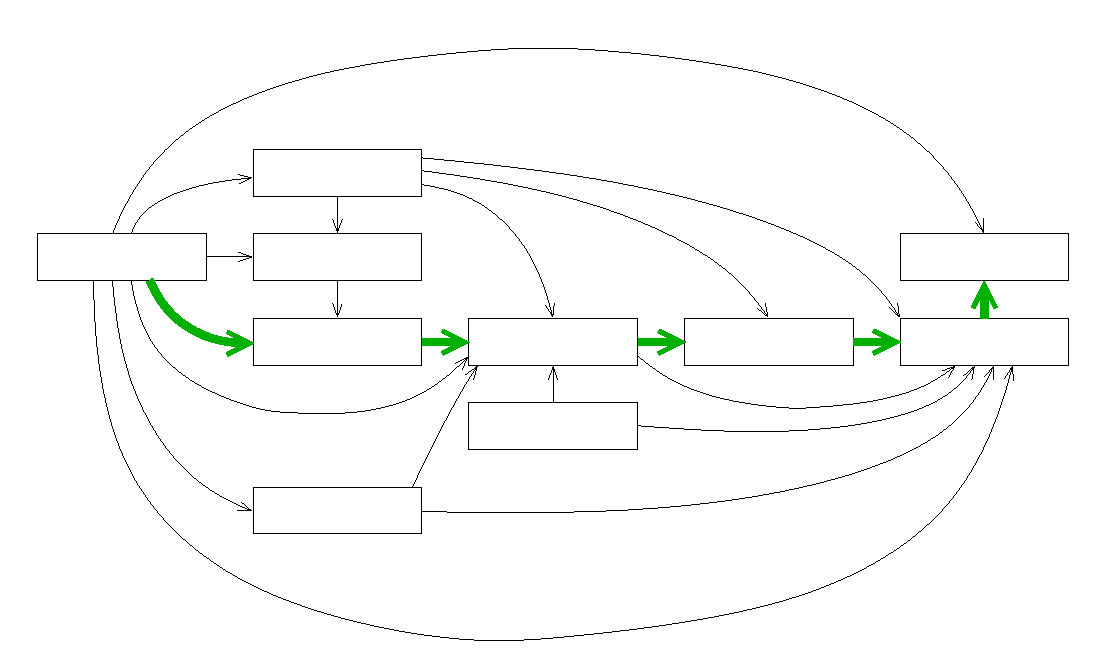
\includegraphics{getdp-struct}%
\end{picture}%
\setlength{\unitlength}{3947sp}%
%
\begingroup\makeatletter\ifx\SetFigFont\undefined%
\gdef\SetFigFont#1#2#3#4#5{%
  \reset@font\fontsize{#1}{#2pt}%
  \fontfamily{#3}\fontseries{#4}\fontshape{#5}%
  \selectfont}%
\fi\endgroup%
\begin{picture}(8552,4992)(300,-6402)
\put(1126,-3361){\makebox(0,0)[b]{\smash{\SetFigFont{10}{12.0}{\rmdefault}{\mddefault}{\updefault}{\color[rgb]{0,0,0}\code{Group}}%
}}}
\put(2851,-2686){\makebox(0,0)[b]{\smash{\SetFigFont{10}{12.0}{\rmdefault}{\mddefault}{\updefault}{\color[rgb]{0,0,0}\code{Function}}%
}}}
\put(2851,-3361){\makebox(0,0)[b]{\smash{\SetFigFont{10}{12.0}{\rmdefault}{\mddefault}{\updefault}{\color[rgb]{0,0,0}\code{Constraint}}%
}}}
\put(2851,-4036){\makebox(0,0)[b]{\smash{\SetFigFont{10}{12.0}{\rmdefault}{\mddefault}{\updefault}{\color[rgb]{0,0,0}\code{FunctionSpace}}%
}}}
\put(2851,-5386){\makebox(0,0)[b]{\smash{\SetFigFont{10}{12.0}{\rmdefault}{\mddefault}{\updefault}{\color[rgb]{0,0,0}\code{Jacobian}}%
}}}
\put(4576,-4711){\makebox(0,0)[b]{\smash{\SetFigFont{10}{12.0}{\rmdefault}{\mddefault}{\updefault}{\color[rgb]{0,0,0}\code{Integration}}%
}}}
\put(4576,-4036){\makebox(0,0)[b]{\smash{\SetFigFont{10}{12.0}{\rmdefault}{\mddefault}{\updefault}{\color[rgb]{0,0,0}\code{Formulation}}%
}}}
\put(6301,-4036){\makebox(0,0)[b]{\smash{\SetFigFont{10}{12.0}{\rmdefault}{\mddefault}{\updefault}{\color[rgb]{0,0,0}\code{Resolution}}%
}}}
\put(8026,-3361){\makebox(0,0)[b]{\smash{\SetFigFont{10}{12.0}{\rmdefault}{\mddefault}{\updefault}{\color[rgb]{0,0,0}\code{PostOperation}}%
}}}
\put(8026,-4036){\makebox(0,0)[b]{\smash{\SetFigFont{10}{12.0}{\rmdefault}{\mddefault}{\updefault}{\color[rgb]{0,0,0}\code{PostProcessing}}%
}}}
\end{picture}
}
\end{center}

\end{slide}

\begin{slide}

\begin{center}
Particular data of a problem\\
\medskip
\scalebox{0.54}{\begin{picture}(0,0)%
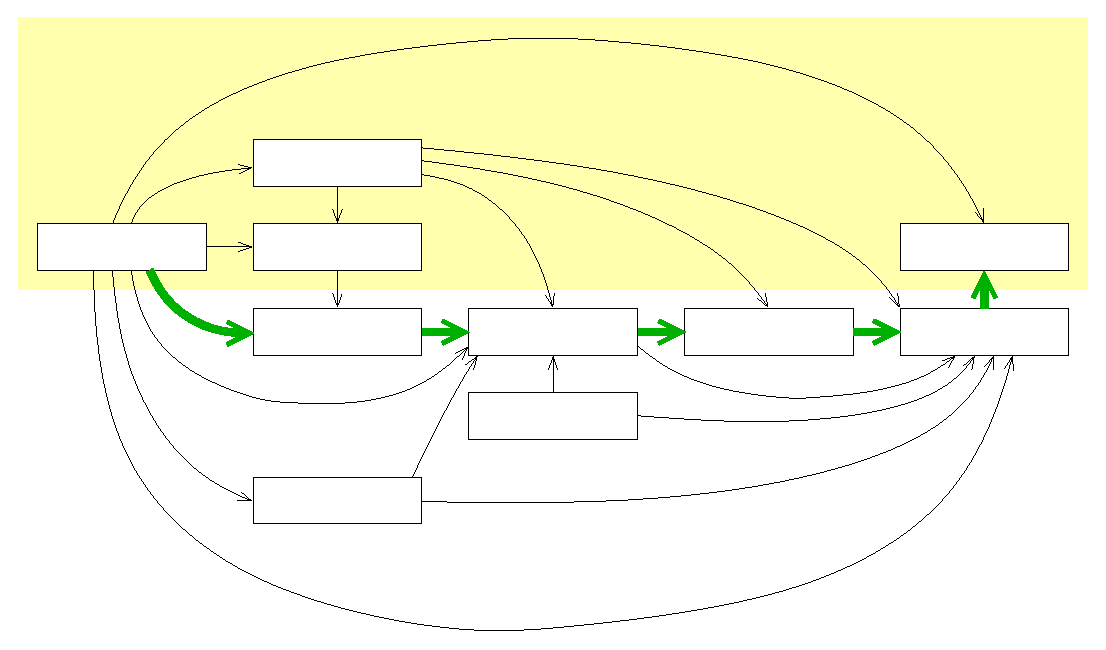
\includegraphics{getdp-struct-box}%
\end{picture}%
\setlength{\unitlength}{3947sp}%
%
\begingroup\makeatletter\ifx\SetFigFont\undefined%
\gdef\SetFigFont#1#2#3#4#5{%
  \reset@font\fontsize{#1}{#2pt}%
  \fontfamily{#3}\fontseries{#4}\fontshape{#5}%
  \selectfont}%
\fi\endgroup%
\begin{picture}(8552,4917)(300,-6402)
\put(1126,-3361){\makebox(0,0)[b]{\smash{\SetFigFont{10}{12.0}{\rmdefault}{\mddefault}{\updefault}{\color[rgb]{0,0,0}\code{Group}}%
}}}
\put(2851,-2686){\makebox(0,0)[b]{\smash{\SetFigFont{10}{12.0}{\rmdefault}{\mddefault}{\updefault}{\color[rgb]{0,0,0}\code{Function}}%
}}}
\put(2851,-3361){\makebox(0,0)[b]{\smash{\SetFigFont{10}{12.0}{\rmdefault}{\mddefault}{\updefault}{\color[rgb]{0,0,0}\code{Constraint}}%
}}}
\put(2851,-4036){\makebox(0,0)[b]{\smash{\SetFigFont{10}{12.0}{\rmdefault}{\mddefault}{\updefault}{\color[rgb]{0,0,0}\code{FunctionSpace}}%
}}}
\put(2851,-5386){\makebox(0,0)[b]{\smash{\SetFigFont{10}{12.0}{\rmdefault}{\mddefault}{\updefault}{\color[rgb]{0,0,0}\code{Jacobian}}%
}}}
\put(4576,-4711){\makebox(0,0)[b]{\smash{\SetFigFont{10}{12.0}{\rmdefault}{\mddefault}{\updefault}{\color[rgb]{0,0,0}\code{Integration}}%
}}}
\put(4576,-4036){\makebox(0,0)[b]{\smash{\SetFigFont{10}{12.0}{\rmdefault}{\mddefault}{\updefault}{\color[rgb]{0,0,0}\code{Formulation}}%
}}}
\put(6301,-4036){\makebox(0,0)[b]{\smash{\SetFigFont{10}{12.0}{\rmdefault}{\mddefault}{\updefault}{\color[rgb]{0,0,0}\code{Resolution}}%
}}}
\put(8026,-3361){\makebox(0,0)[b]{\smash{\SetFigFont{10}{12.0}{\rmdefault}{\mddefault}{\updefault}{\color[rgb]{0,0,0}\code{PostOperation}}%
}}}
\put(8026,-4036){\makebox(0,0)[b]{\smash{\SetFigFont{10}{12.0}{\rmdefault}{\mddefault}{\updefault}{\color[rgb]{0,0,0}\code{PostProcessing}}%
}}}
\end{picture}
}\\
\medskip
Method of resolution (``black box'')
\end{center}

\end{slide}

% ---------------------------------------------------------------------------

\smallgetdp{fig/getdp-struct-group.tex}

\chapter{\code{Group}: defining topological entities}

\begin{slide}

\mybox{colbox}{11\semcm}{
  \begin{slideitemize}
  \item Regions
  \item Functions on Regions (nodes, edges, edges of tree, ...)
  \end{slideitemize}
}

\bigskip
\begin{syntax}
Air = Region[1]; \CC{elementary group (linked with the mesh)}
Core = Region[2];
Omega = Region[\{Air, Core\}];
Nodes = NodesOf[Omega]; \CC{function group}
\end{syntax}

\end{slide}

% ---------------------------------------------------------------------------

\smallgetdp{fig/getdp-struct-function.tex}

\chapter{\code{Function}: defining expressions}

\begin{slide}

\mybox{colbox}{11\semcm}{
  \begin{slideitemize}
  \item Physical characteristics
  \item Time functions
  \item Various other functions (natural contraints, ...)
  \end{slideitemize}
}

\bigskip
\begin{syntax}
mu0 = 4.e-7*Pi; f = 50; \CC{constants}
mu[Air] = mu0; 
mu[Core] = mu0 + 1/(100+100*$1^6); \CC{argument ($1 <- b)}
TimeFct[] = Cos[2*Pi*f*$Time] * Exp[-$Time/0.012]; \CC{current value}
\end{syntax}

\end{slide}

% ---------------------------------------------------------------------------

\smallgetdp{fig/getdp-struct-constraint.tex}

\chapter{\code{Constraint}: specifying constraints}

\begin{slide}

\mybox{colbox}{11\semcm}{
  \begin{slideitemize}
  \item Boundary conditions (classical, connection)
  \item Initial conditions
  \item Topology of circuits with lumped elements
  \item Other constraints (on local and global quantities)
  \end{slideitemize}
}

\bigskip
\begin{syntax}
\{ Name Dirichlet; Type Assign; \CC{boundary conditions}
  Case \{ \{ Region Surface0; Value 0; \}
         \{ Region Surface1; Value 1; \} \}
\}
\end{syntax}

\end{slide}

\background{7\semcm}{-2.5\semcm}{\scalebox{0.65}{\begin{picture}(0,0)%
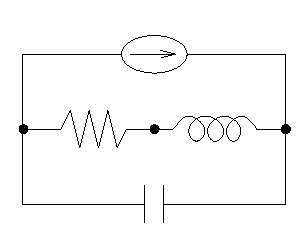
\includegraphics{getdp-rlccircuit}%
\end{picture}%
\setlength{\unitlength}{3947sp}%
%
\begingroup\makeatletter\ifx\SetFigFont\undefined%
\gdef\SetFigFont#1#2#3#4#5{%
  \reset@font\fontsize{#1}{#2pt}%
  \fontfamily{#3}\fontseries{#4}\fontshape{#5}%
  \selectfont}%
\fi\endgroup%
\begin{picture}(2387,1794)(1923,-4573)
\put(4310,-3856){\makebox(0,0)[lb]{\smash{\SetFigFont{10}{12.0}{\rmdefault}{\mddefault}{\updefault}{\color[rgb]{0,0,0}$2$}%
}}}
\put(3601,-3586){\makebox(0,0)[lb]{\smash{\SetFigFont{10}{12.0}{\rmdefault}{\mddefault}{\updefault}{\color[rgb]{0,0,0}$L_1$}%
}}}
\put(3076,-2944){\makebox(0,0)[lb]{\smash{\SetFigFont{10}{12.0}{\rmdefault}{\mddefault}{\updefault}{\color[rgb]{0,0,0}$E_1$}%
}}}
\put(2615,-3527){\makebox(0,0)[lb]{\smash{\SetFigFont{10}{12.0}{\rmdefault}{\mddefault}{\updefault}{\color[rgb]{0,0,0}$R_1$}%
}}}
\put(1923,-3869){\makebox(0,0)[lb]{\smash{\SetFigFont{10}{12.0}{\rmdefault}{\mddefault}{\updefault}{\color[rgb]{0,0,0}$1$}%
}}}
\put(3119,-3710){\makebox(0,0)[lb]{\smash{\SetFigFont{10}{12.0}{\rmdefault}{\mddefault}{\updefault}{\color[rgb]{0,0,0}$3$}%
}}}
\put(3086,-4138){\makebox(0,0)[lb]{\smash{\SetFigFont{10}{12.0}{\rmdefault}{\mddefault}{\updefault}{\color[rgb]{0,0,0}$C_1$}%
}}}
\end{picture}
}}

\begin{slide}

\begin{syntax}
\{ Name Current; Type Assign; \CC{constraints on global quantities}
  Case \{ 
    \{ Region Inductor1; Value 1000; TimeFunction TimeFct[]; \} 
  \} 
\}

\{ Name ElectricalCircuit; Type Network; \CC{circuit}
  Case Circuit1 \{ 
    \{ Region E1; Branch \{1,2\}; \}
    \{ Region R1; Branch \{1,3\}; \}
    \{ Region L1; Branch \{3,2\}; \}
    \{ Region C1; Branch \{1,2\}; \}
  \}
\}
\end{syntax}

\end{slide}


% ---------------------------------------------------------------------------

\smallgetdp{fig/getdp-struct-functionspace.tex}

\chapter{\code{FunctionSpace}: building function spaces}

\begin{slide}

\mybox{colbox}{11\semcm}{
  \begin{slideitemize}
  \item Various quantity types (0, 1, 2, 3-forms, scalar, vector)
  \item Various basis functions (associated with nodes, edges, facets,
  volumes) of various orders
  \item Coupling of fields and potentials ($T$-$\Omega$, $\vec{h}$-$\phi$,
  $\vec{a}$-$v$, ...)
  \item Definition of global quantities (fluxes, circulations: current,
  voltage, m.m.f., ...)
  \item Essential constraints (boundary and gauge conditions, ...)
  \end{slideitemize}
}

\rput(0.75\textwidth,4\semcm){\begin{picture}(0,0)%
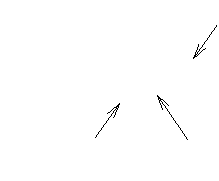
\includegraphics{getdp-sum}%
\end{picture}%
\setlength{\unitlength}{3947sp}%
%
\begingroup\makeatletter\ifx\SetFigFont\undefined%
\gdef\SetFigFont#1#2#3#4#5{%
  \reset@font\fontsize{#1}{#2pt}%
  \fontfamily{#3}\fontseries{#4}\fontshape{#5}%
  \selectfont}%
\fi\endgroup%
\begin{picture}(1742,1435)(2020,-4818)
\put(2020,-4668){\makebox(0,0)[lb]{\smash{\SetFigFont{10}{12.0}{\rmdefault}{\mddefault}{\updefault}{\color[rgb]{0,0,0}\small Geometrical}%
}}}
\put(2162,-4818){\makebox(0,0)[lb]{\smash{\SetFigFont{10}{12.0}{\rmdefault}{\mddefault}{\updefault}{\color[rgb]{0,0,0}\small entities}%
}}}
\put(3220,-4668){\makebox(0,0)[lb]{\smash{\SetFigFont{10}{12.0}{\rmdefault}{\mddefault}{\updefault}{\color[rgb]{0,0,0}\small Degrees of}%
}}}
\put(3321,-4817){\makebox(0,0)[lb]{\smash{\SetFigFont{10}{12.0}{\rmdefault}{\mddefault}{\updefault}{\color[rgb]{0,0,0}\small freedom}%
}}}
\put(3244,-3488){\makebox(0,0)[lb]{\smash{\SetFigFont{10}{12.0}{\rmdefault}{\mddefault}{\updefault}{\color[rgb]{0,0,0}\small Basis functions}%
}}}
\put(2176,-4036){\makebox(0,0)[lb]{\smash{\SetFigFont{10}{12.0}{\rmdefault}{\mddefault}{\updefault}{\color[rgb]{0,0,0}$f(\vec{x})=\sum_{i\in E}f_i w_i(\vec{x})$}%
}}}
\end{picture}
}

\end{slide}

\background{}{}{}

\begin{slide}

\begin{syntax}
\{ Name H1 ; Type Form0 ; \CC{discrete function space for H1}
  BasisFunction \{
    \{ Name wi ; NameOfCoef fi ; Function BF_Node ; \CC{order 1}
      Support Omega ; Entity NodesOf[ All ] ; \}
    \{ Name wi2 ; NameOfCoef fi2 ; Function BF_Node_2E ;  \CC{order 2}
      Support Omega ; Entity EdgesOf[ All ] ; \}
  \}
  Constraint \{
    \{ NameOfCoef fi ; \CC{cf. 'Constraint'}
      EntityType NodesOf ; NameOfConstraint Dirichlet ; \}
    \{ NameOfCoef fi2 ;
      EntityType NodesOf ; NameOfConstraint Dirichlet ; \}
  \}
\}
\end{syntax}

\end{slide}


% ---------------------------------------------------------------------------

\smallgetdp{fig/getdp-struct-jacobian.tex}

\chapter{\code{Jacobian}: defining jacobian methods}

\begin{slide}

\mybox{colbox}{11\semcm}{
  \begin{slideitemize}
  \item Mapping from reference to real space 
  \item Geometrical transformations (axisymmetric transformation, infinite
  domains, ...)
  \end{slideitemize}
}

\bigskip
\begin{syntax}
\{ Name Jacobian1 ;
  Case \{ \CC{piece-wise defined on groups}
    \{ Region OmegaInf; Jacobian VolSphShell \{Rint, Rext\}; \}
    \{ Region OmegaAxi; Jacobian VolAxi; \}
    \{ Region All; Jacobian Vol ; \}
  \}
\}
\end{syntax}

\end{slide}

% ---------------------------------------------------------------------------

\smallgetdp{fig/getdp-struct-integration.tex}

\chapter{\code{Integration}: defining integration methods}

\begin{slide}

\bigskip
\bigskip
\mybox{colbox}{11\semcm}{
  \begin{slideitemize}
  \item Various numeric and analytic integration methods
  \item Criterion-based selection
  \end{slideitemize}
}

\bigskip
\bigskip
\begin{syntax}
\{ Name Integration1 ; Criterion Test[]; \CC{combination of methods}
  Case \{ 
    \{ Type Gauss ;
      Case \{ \{ GeoElement Triangle ; NumberOfPoints 12; \}
             \{ GeoElement Tetrahedron; NumberOfPoints 15; \} \} \}
    \{ Type Analytic ; \}
  \} 
\}
\end{syntax}

\end{slide}

% ---------------------------------------------------------------------------

\smallgetdp{fig/getdp-struct-formulation.tex}

\chapter{\code{Formulation}: building equations}

\begin{slide}

\mybox{colbox}{11\semcm}{
  \begin{slideitemize}
  \item Various formulation types: FEM, BEM, circuit equations, ...
  \item Symbolic expression of equations: volume and surface integral
  terms, collocation
  \item Involves local, global and integral quantities based on function
  spaces
  \end{slideitemize}
}

\begin{syntax}
Equation \{
  Galerkin \{ DtDt [ epsilon[] * Dof\{e\} , \{e\} ]; ... \}
  Galerkin \{ [ 1/mu[] * Dof\{Curl e\} , \{Curl e\} ]; ... \}
\}
\end{syntax}

\rput(0.8\textwidth,6\semcm)
     {$\partial_t^2\ivol{\epsilon\vec{e}}{\vec{e}} + 
       \ivol{\mu^{-1}\Curl{\vec{e}}}{\Curl{\vec{e}}'}=0$}

\end{slide}

% ---------------------------------------------------------------------------

\smallgetdp{fig/getdp-struct-resolution.tex}

\chapter{\code{Resolution}: solving systems of equations}

\begin{slide}

\mybox{colbox}{10\semcm}{
  \begin{slideitemize}
  \item Description of a sequence of operations
  \item Time loops (with time step adaptation)
  \item Nonlinear iterative loops (e.g.\ fixed point or Newton-Raphson methods)
  \item Coupled problems (e.g.\ magneto-thermal coupling)
  \item Linking of various resolution steps (e.g.\ pre-computation of source
  fields) 
  \end{slideitemize}
}

\rput(0.8\textwidth,4\semcm){\parbox{12\semcm}{
\begin{syntax}
Operation\{\\
\hspace*{1em}InitSolution[A];\\
\hspace*{1em}TimeLoopTheta[tmin,tmax,dt,1]\{\\
\hspace*{2em}Generate[A]; Solve[A];\\
\hspace*{2em}If[Save[]]\{ SaveSolution[A]; \}\\
\hspace*{1em}\}\\
\}
\end{syntax}
}}

\end{slide}

% ---------------------------------------------------------------------------

\smallgetdp{fig/getdp-struct-postprocessing.tex}

\chapter{\code{PostProcessing}: exploiting computational data}

\begin{slide}

\mybox{colbox}{11\semcm}{
  \begin{slideitemize}
  \item ``Front-end'' to computational data
  \item Piece-wise definition of any quantity of interest
  \item Local or integral evaluation
  \end{slideitemize}
}

\bigskip
\begin{syntax}
Quantity \{
  \{ Name Induction;
    Value \{ Local \{ [ -mu[]*\{Grad phi\} ]; In Omega; \}
            Local \{ [ -\{dGreen\} ]; In BEM; \} \}
\}
\end{syntax}


\end{slide}

% ---------------------------------------------------------------------------

\smallgetdp{fig/getdp-struct-postoperation.tex}

\chapter{\code{PostOperation}: exporting results}

\begin{slide}

\mybox{colbox}{11\semcm}{
  \begin{slideitemize}
  \item Evaluation of post-processing quantities (e.g.\ maps, cuts, local or
  global evaluation, ...)
  \item Operations on post-processing quantities (sorting, smoothing,
  adaptation, ...) 
  \item Various output formats (e.g.\ space or time oriented, text, binary,
  ...) 
  \end{slideitemize}
}

\bigskip
\begin{syntax}
Print[ Induction, OnElementsOf Omega, File "b.pos", Format Gmsh ] ;
Print[ Induction, OnLine \{\{0,0,0\}\{1,0,0\}\} \{100\}, File "b.cut" ] ;
\end{syntax}

\end{slide}


\background{}{}{}


% $Id: gmsh.tex,v 1.5 2001-06-13 16:00:29 geuzaine Exp $

\chapter{}

\begin{slide}

\slidepagestyle{reduced}

\begin{center}
\bigtitle{Gmsh --- Geometry, mesh, solver integration
and visualization}\\
\ifthenelse{\boolean{fulltitle}}{
\bigskip\bigskip
\begin{minipage}{0.5\textwidth}\center
\mediumtitle{Christophe Geuzaine}\\
\bigskip
\smalltitle{Dept. of Electrical Engineering}\\
\smalltitle{Montefiore Institute B28, Sart Tilman}\\
\smalltitle{University of Li�ge}\\
\smalltitle{B-4000 Li�ge (BELGIUM)}
\end{minipage}%
\begin{minipage}{0.5\textwidth}\center
\mediumtitle{Jean-Fran�ois Remacle}\\
\bigskip
\smalltitle{Scientific Computation Research Center}\\
\smalltitle{Rensselaer Polytechnic Insitute}\\
\smalltitle{CII 110 8th Street}\\
\smalltitle{Troy, New York 12180-3590 (USA)}
\end{minipage}}
\end{center}

\end{slide}

% ---------------------------------------------------------------------------
\part{Gmsh}
% ---------------------------------------------------------------------------

\chapter{Finite element methods in practice}

\begin{slide}

Four main steps:
\begin{slideitemize}
\item \emph{Geometry}: CAD sofware
\item \emph{Mesh}: structured or unstructed mesh generator
\item \emph{Solver}: GetDP :-)
\item \emph{Post-processing}: various visualization tools (2D and 3D)
\end{slideitemize}

Most of the time spent solving a problem is \emph{not} in the solver step!

\end{slide}

% ---------------------------------------------------------------------------

\background{7\semcm}{4.2\semcm}
           {\scalebox{0.3}{\input{fig/gmsh-geo.tex}}}

\chapter{Geometry description}

\begin{slide}

Constructive:


Parametric (scriptable):



\end{slide}

% ---------------------------------------------------------------------------

\background{7\semcm}{4.2\semcm}
           {\scalebox{0.3}{\input{fig/gmsh-mesh.tex}}}

\chapter{Mesh generation}

\begin{slide}

\begin{slideitemize}
\item \emph{Structured} (transfinite, elliptic, hyperbolic)
\item \emph{Unstructured} (Delaunay triangles/tetrahedra)
\begin{enumerate}
\item 
mesh of a box including the convex polygon/polyhedron resulting from
curves/surfaces discretization
\item
initial mesh by insertion of curves/surfaces nodes by the Bowyer algorithm
\item 
boundary restoration to force presence of all edges/faces
\item 
suppression of undesired triangles/tetrahedra
\item
new node insertions by the Bowyer algorithm until the characteristic size of
each simplex $\leq$ characteristic length field evaluated at the center of
its circumscribed circle/sphere.
\item
mesh post-processing and quality enforcement by node relocation and edge
swapping
\end{enumerate}
\end{slideitemize}

\end{slide}

% ---------------------------------------------------------------------------

\background{7\semcm}{4.2\semcm}
           {\scalebox{0.3}{\input{fig/gmsh-solver.tex}}}

\chapter{Solver integration}

\begin{slide}

\begin{minipage}{0.45\textwidth}
\emph{Batch}:
\begin{slideitemize}
\item Advanced users
\item No graphical overhead
\item Easily scriptable
\end{slideitemize}
$\rightarrow$ for heavy problems
\end{minipage}%
\begin{minipage}{0.1\textwidth}
vs.
\end{minipage}%
\begin{minipage}{0.45\textwidth}
\emph{Interactive}:
\begin{slideitemize}
\item Smoother learning curve
\item Better integration
\item Faster for testing
\end{slideitemize}
$\rightarrow$ for testing/learning
\end{minipage}%

\end{slide}

\begin{slide}

Example: integration of GetDP into higher level toolboxes (visualization,
optimization, etc.):
\begin{slideitemize}
\item \emph{High level}: Commercial applications (Matlab, Mathematica, ...),
shell scripts (bash, Perl, Python, ...), other programming languages (C,
C++, ...) 

$\rightarrow$ \emph{system calls}
\item \emph{Medium level}: Home-grown applications (Gmsh, ...), shell scripts
(Perl, Python, ...), other programming languages (C, C++, ...) 

$\rightarrow$ \emph{sockets}
\item \emph{Low level}: programming languages (C, C++, ...) 

$\rightarrow$ \emph{source code}
\end{slideitemize}

\end{slide}

% ---------------------------------------------------------------------------

\background{7\semcm}{4.2\semcm}
           {\scalebox{0.3}{\input{fig/gmsh-postpro.tex}}}

\chapter{Post-processing}

\begin{slide}

Scriptable:

Modular:


\end{slide}

% ---------------------------------------------------------------------------


% $Id: examples.tex,v 1.12 2001-07-18 09:09:51 geuzaine Exp $

%
% WARNING:
%
% If \bigpictures is set to 1, the pictures must have been checked out
% (cvs module name is getdp-picts) in the ../../../getdp-picts directory.
%

% ---------------------------------------------------------------------------
\part{GetDP/Gmsh examples}
% ---------------------------------------------------------------------------

\begin{slide}

\slidepagestyle{none}

\begin{center}
\bigtitle{Examples}\\
\ifnum\fulltitle=1\par\bigskip\bigskip
\mediumtitle{Patrick Dular and Christophe Geuzaine}\\
\bigskip
\smalltitle{Department of Electrical Engineering}\\
\smalltitle{Montefiore Institute B28, Sart Tilman Campus}\\
\smalltitle{University of Li�ge}\\
\smalltitle{B-4000 Li�ge (BELGIUM)}
\fi
\end{center}

\end{slide}

% ---------------------------------------------------------------------------

\chapter{Magnetostatics}

\ifnum\bigpictures=1

\begin{slide}

\begin{center}
\includegraphics[width=0.37\textwidth]{getdp-picts/ind1}%
\includegraphics[width=0.37\textwidth]{getdp-picts/ind2}

\includegraphics[width=0.37\textwidth]{getdp-picts/ind3}%
\includegraphics[width=0.37\textwidth]{getdp-picts/ind4}
\end{center}

\end{slide}

\fi

\begin{slide}

\mybox{colbox}{0.98\textwidth}{
\begin{equation*}
\Curl{\vec{h}} = \vec{j} ,\quad
\Div{\vec{b}} = 0 \quad\text{and}\quad
\vec{b} = \mu \vec{h} + \mu_0 \vec{h}_m 
\end{equation*}
\begin{equation*}
\begin{split}
\xymatrix{
 \color{colpos}\phi    \ar@{->}[r]^-{\GradSymb_h}  &
 \vec{h} \ar@{->}[r]^-{\CurlSymb_h} \ar@{<->}[d]^{\mu} &
 \vec{j} \ar@{->}[r]^-{\DivSymb_h}   &
 0 \\
 0       \ar@{<-}[r]^-{\DivSymb_e}&
 \vec{b} \ar@{<-}[r]^-{\CurlSymb_e}&
 \color{colpos}\vec{a} 
}
\end{split}
\end{equation*}
}

\begin{slideitemize}
\item Weak form of Gauss' law: 
\begin{equation*}
% \ivol{\Div{\vec{b}}}{\phi'} = 0 \Rightarrow
\ivol{\vec{b}}{\Grad{\phi'}} + \isur{\psca{\vec{n}}{\vec{b}}}{\phi'} 
= 0
\quad \forall\phi'\in\Hone[_0]{\Omega}
\end{equation*}

\item Weak form of Amp�re's law:
\begin{equation*}
% \ivol{\Curl{\vec{h}}}{\vec{a}'} = \ivol{\vec{j}}{\vec{a}'} \Rightarrow
\ivol{\vec{h}}{\Curl{\vec{a}'}} + \isur{\pvec{\vec{n}}{\vec{h}}}{\vec{a}'}
= \ivol{\vec{j}}{\vec{a}'} 
\quad \forall\vec{a}'\in\Hcurl[_0]{\Omega}
\end{equation*}

\end{slideitemize}

\end{slide}

% ---------------------------------------------------------------------------

\chapter{Magnetostatics: $\vec{b}$-conforming}

\begin{slide}

\mybox{colbox}{0.98\textwidth}{
\begin{center}
\emph{Vector potential} formulation
\begin{equation*}
\vec{b} = \Curl{\vec{a}}
\end{equation*}
\end{center}
}

\begin{center}
$\Downarrow$\\
Weak form of Amp�re's law\\
$\Downarrow$\\
$\displaystyle\ivol{\mu^{-1}\Curl{\vec{a}}}{\Curl{\vec{a}'}} 
= \ivol{\vec{j}}{\vec{a}'} ,
\quad\forall\vec{a}'\in\Hcurl[_0]{\Omega}$
\end{center}

\bigskip
NB: gauge for $\vec{a}$, ...

\end{slide}

\ifnum\bigpictures=1

\background{7\semcm}{0\semcm}{\includegraphics[width=0.38\textwidth]{getdp-picts/ind1}}

\fi

\begin{slide}

\begin{smallsyntax}
Group \{
  Core = #1; Inductor = #2; SkinInductor = #3, Air = #4;
  Omega = Region[\{Core, Inductor, Air\}];
\}
Function \{
  mu0 = 4.e-7 * Pi; mur = 1000;
  mu[ Core ] = mur * mu0;
  mu[ Region[\{Air, Inductor\}] ] = mu0;
  j[ Inductor ] = ...; //to be defined
\}
Constraint \{
  \{ Name a; 
    Case \{ 
      \{ Region CL_a0; Value 0; \}
    \}
  \}
\}
\end{smallsyntax}

\end{slide}

\background{}{}{}

\begin{slide}

\begin{smallsyntax}
FunctionSpace \{
  \{ Name Hcurl; Type Form1; \CC{vector potential}
    BasisFunction \{
      \{ Name se;  NameOfCoef ae; Function BF_Edge; Support Omega; 
        Entity EdgesOf[All]; \} \CC{associated with the edges of the mesh}
    \}
    Constraint \{ \CC{essential constraint + gauge (unicity)}
      \{ NameOfCoef ae;  EntityType EdgesOf; NameOfConstraint a; \}
      \{ NameOfCoef ae;  EntityType EdgesOfTreeIn;
        EntitySubType StartingOn; NameOfConstraint Gauge; \}
    \}
  \}
\}
\end{smallsyntax}

\end{slide}

\begin{slide}

\begin{smallsyntax}
Formulation \{
  \{ Name MagSta_a; Type FemEquation;
    Quantity \{ 
      \{ Name a; Type Local; NameOfSpace Hcurl; \}
    \}
    Equation \{
      Galerkin \{ [ 1/mu[] * Dof\{Curl a\} , \{Curl a\} ]; 
                 In Omega; Integration I1; Jacobian JVol; \}
      Galerkin \{ [ -j[] , \{a\} ]; 
                 In Inductor; Integration I1; Jacobian JVol; \}
    \}
  \}
\}
\end{smallsyntax}

\end{slide}

\begin{slide}

\begin{smallsyntax}
Resolution \{
  \{ Name MagSta_a;
    System \{
      \{ Name A; NameOfFormulation MagSta_a; \}
    \}
    Operation \{ Generate[A]; Solve[A]; SaveSolution[A]; \}
  \}
\}
PostProcessing \{
  \{ Name test; NameOfFormulation MagSta_a;
    Quantity \{
      \{ Name a; Value \{ Local\{ [ \{a\} ]; In Omega; \} \} \}
      \{ Name normb; Value \{ Local\{ [ Norm[\{d a\}] ]; Omega; \} \} \}
    \}
  \}
\}
\end{smallsyntax}

\end{slide}

\begin{slide}

Magnetodynamics?

Additional term in the formulation: 

\begin{smallsyntax}
      Galerkin \{ DtDof [ sigma[] * Dof\{a\} , \{a\} ]; 
                 In Core; Integration I1; Jacobian JVol; \}   
\end{smallsyntax}

New resolution:
\begin{smallsyntax}
  \{ Name MagDyn_a_t; \CC{time domain}
    System \{
      \{ Name A; NameOfFormulation MagDyn_a; \}
    \}
    Operation \{ 
      InitSolution[A]
      TimeLoopTheta[0,20/50,0.1/50,1] \{ \CC{tmin,tmax,dt,theta}
        Generate[A]; Solve[A]; SaveSolution[A];
      \}
    \}
  \}
\end{smallsyntax}


\end{slide}

% ---------------------------------------------------------------------------

\chapter{Magnetostatics: $\vec{h}$-conforming}

\begin{slide}

\mybox{colbox}{0.98\textwidth}{
\begin{center}
\emph{Magnetic field conforming} formulation
\begin{equation*}
\vec{h} = \vec{h}_s+\vec{h}_r ,\quad\text{with}\quad
\Curl{\vec{h}_s} = \vec{j}     \quad\text{and}\quad
\vec{h}_r = -\Grad{\phi}
\end{equation*}
\end{center}
}

\begin{center}
$\Downarrow$\\
Weak form of Gauss law\\
$\Downarrow$\\
$\displaystyle\ivol{\mu(-\Grad{\phi}+\vec{h}_s)}{\Grad{\phi'}} 
= 0 ,
\quad \forall\phi'\in\Hone[_0]{\Omega}$
\end{center}

\bigskip
NB: choice of source field $\vec{h}_s$, treatment of multiply connected
$\Omega$, ...

\end{slide}

\begin{slide}

\begin{smallsyntax}
FunctionSpace \{
  \{ Name H1; Type Form0; \CC{scalar potential}
    BasisFunction \{
      \{ Name sn; NameOfCoef phin; Function BF_Node; Support Omega; 
        Entity NodesOf[All]; \} \CC{associated with the nodes of Omega}
    \}
    Constraint \{ \CC{essential constraint}
      \{ NameOfCoef phin; EntityType NodesOf; NameOfConstraint phi; \}
    \}
  \}
\}
\end{smallsyntax}

\end{slide}

\begin{slide}

\begin{smallsyntax}
Formulation \{
  \{ Name MagSta_phi; Type FemEquation;
    Quantity \{
      \{ Name phi; Type Local; NameOfSpace H1; \}
      \{ Name hs; Type Local; NameOfSpace Hcurl_s; \} \CC{patience...}
    \}
    Equation \{
      Galerkin \{ [ mu[] * \{hs\} , \{Grad phi\} ];
                 In Omega; Integration I1; Jacobian JVol;  \}
      Galerkin \{ [ mu[] * Dof\{Grad phi\} , \{Grad phi\} ]; 
                 In Omega; Integration I1; Jacobian JVol;  \}
    \}
  \}
\}

\end{smallsyntax}

\end{slide}

\begin{slide}[1.05\slidewidth,\slideheight]

\begin{smallsyntax}
FunctionSpace \{
  \{ Name Hcurl_s; Type Form1; \CC{space for the source field}
    BasisFunction \{
      \{ Name se; NameOfCoef he; Function BF_Edge; Support Inductor; 
        Entity EdgesOf[All, Not SkinInductor]; \}
      \{ Name sc; NameOfCoef Ic; Function BF_GradGroupOfNodes; 
        Support Transition; Entity GroupsOfNodesOf[Cut]; \}
      \{ Name sc; NameOfCoef Icc; Function BF_GroupOfEdges; 
        Support Inductor; Entity ...; \}
    \}
    Constraint \{
      \{ NameOfCoef he; EntityType EdgesOfTreeIn;
        EntitySubType StartingOn; NameOfConstraint Gauge; \}
      \{ NameOfCoef Ic; EntityType GroupsOfNodesOf; NameOfConstraint I; \}
      \{ NameOfCoef Icc; EntityType GroupsOfNodesOf; NameOfConstraint I; \}
    \}
  \}
\}
\end{smallsyntax}

%... -> GroupsOfEdgesOf[Cut, InSupport ElementsOf[SkinInductor, OnOneSideOf Cut] ]

\end{slide}

\begin{slide}

\begin{smallsyntax}
Formulation \{
  \{ Name MagSta_hs; Type FemEquation;
    Quantity \{
      \{ Name hs; Type Local; NameOfSpace Hcurl_hs; \}
    \}
    Equation \{
      Galerkin \{ [ Dof\{Curl hs\} , \{Curl hs\} ];
                 In Omega; Integration I1; Jacobian JVol; \}
      Galerkin \{ [ -j[] , \{d hs\} ];
                 In Omega; Integration I1; Jacobian JVol; \}
    \}
  \}
\}
\end{smallsyntax}

% Resolution \{ \CC{link pre-computation of source field}
%   \{ Name MagSta_h;
%     System \{
%       \{ Name Hs; NameOfFormulation MagSta_hs; \}
%       \{ Name Phi; NameOfFormulation MagSta_phi; \}
%     \}
%     Operation \{ 
%       Generate[Hs]; Solve[Hs]; SaveSolution[Hs];
%       Generate[Phi]; Solve[Phi]; SaveSolution[Phi];
%     \}
%   \}
% \}

\end{slide}


% ---------------------------------------------------------------------------

\chapter{Magneto-thermal coupling: step by step}

\begin{slide}

\begin{center}
\scalebox{0.8}{\begin{picture}(0,0)%
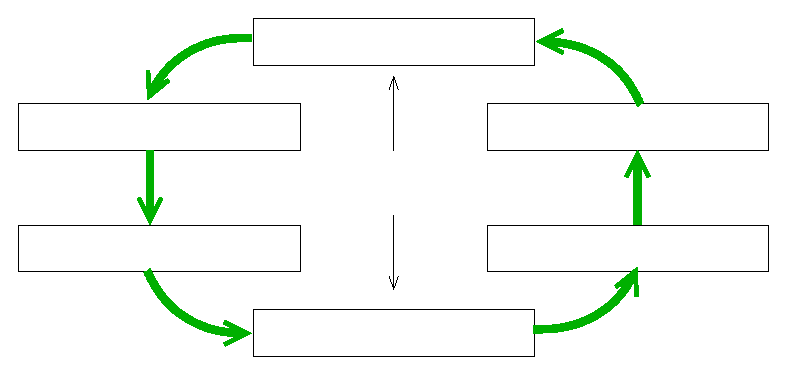
\includegraphics{getdp-magthe}%
\end{picture}%
\setlength{\unitlength}{3947sp}%
%
\begingroup\makeatletter\ifx\SetFigFont\undefined%
\gdef\SetFigFont#1#2#3#4#5{%
  \reset@font\fontsize{#1}{#2pt}%
  \fontfamily{#3}\fontseries{#4}\fontshape{#5}%
  \selectfont}%
\fi\endgroup%
\begin{picture}(6024,2724)(1489,-4723)
\put(4501,-4561){\makebox(0,0)[b]{\smash{\SetFigFont{10}{12.0}{\rmdefault}{\mddefault}{\updefault}{\color[rgb]{0,0,0}\textsf{Thermal problem}}%
}}}
\put(2626,-2911){\makebox(0,0)[b]{\smash{\SetFigFont{10}{12.0}{\rmdefault}{\mddefault}{\updefault}{\color[rgb]{0,0,0}\textsf{Joule power density}}%
}}}
\put(2701,-3886){\makebox(0,0)[b]{\smash{\SetFigFont{10}{12.0}{\rmdefault}{\mddefault}{\updefault}{\color[rgb]{0,0,0}\textsf{Thermal source density}}%
}}}
\put(4501,-3361){\makebox(0,0)[b]{\smash{\SetFigFont{10}{12.0}{\rmdefault}{\mddefault}{\updefault}{\color[rgb]{0,0,0}\textsf{Nonlinear problems}}%
}}}
\put(6376,-3886){\makebox(0,0)[b]{\smash{\SetFigFont{10}{12.0}{\rmdefault}{\mddefault}{\updefault}{\color[rgb]{0,0,0}\textsf{Temperature field}}%
}}}
\put(4501,-2236){\makebox(0,0)[b]{\smash{\SetFigFont{10}{12.0}{\rmdefault}{\mddefault}{\updefault}{\color[rgb]{0,0,0}\textsf{Magnetodynamic problem}}%
}}}
\put(6376,-2911){\makebox(0,0)[b]{\smash{\SetFigFont{10}{12.0}{\rmdefault}{\mddefault}{\updefault}{\color[rgb]{0,0,0}\textsf{Electric physical properties}}%
}}}
\end{picture}
}
\end{center}

\end{slide}

\begin{slide}

\mybox{colbox}{0.98\textwidth}{
\begin{center}
Magnetodynamic formulations
\end{center}
\begin{slideitemize}
\item Adapted function spaces for the fields and potentials involved
\item Boundary conditions
\item Electric circuit coupling, prescribed currents or voltages
\item Nonlinear magnetic characteristics
\end{slideitemize}
}

\parbox{0.1\textwidth}{e.g.}\parbox{0.9\textwidth}{
\begin{gather*}
\ivol[_{\Omega}]{\mu^{-1}\Curl{\vec{a}}}{\Curl{\vec{a}'}} +
\ivol[_{\Omega_c}]{\sigma\partial_t\vec{a}}{\vec{a}'} +
\ivol[_{\Omega_c}]{\sigma\Grad{v}}{\vec{a}'} = 
0, \\
\forall \vec{a}'\in\Hcurl[_0]{\Omega}
\end{gather*}
\begin{equation*}
\partial_t\ivol[_{\Omega}]{\mu\vec{h}}{\vec{h}'} +
\ivol[_{\Omega_c}]{\sigma^{-1}\Curl{\vec{h}}}{\Curl{\vec{h}'}} =
0, \quad
\forall \vec{h}'\in\Hcurl[_0]{\Omega}
\end{equation*}
}

\end{slide}

\begin{slide}

\mybox{colbox}{0.98\textwidth}{
\begin{center}
Thermal formulation
\end{center}
\begin{slideitemize}
\item For example temperature $T$ formulation
\item Essential boundary conditions for $T$
\item Natural boundary conditions for convection and radiation heat flows
\item Nonlinear thermal characteristics
\end{slideitemize}
}

\begin{gather*}
\ivol[_\Omega]                 {\kappa\,\Grad{T}}        {\Grad{T'}}   -
\ivol[_\Omega]             {\rho c_p\,\partial_t T}         {T'}       +
\ivol[_\Omega]                      {p_q}                   {T'}   \\ +
\isur[_{\Gamma_{\text{conv}}}]    {\eta(T-T_0)}                {T'}       +
\isur[_{\Gamma_{\text{rad}}}]{\epsilon\sigma_s(T^4-T_0^4)}  {T'}     = 0  \,, 
\quad\forall T'\in \Hone[_0]{\Omega}
\end{gather*}

% $\sigma$ is Botltzmann's constant
% $\epsilon$ is the emissivity
% $\eta$ is the convection coefficient (2.5->5)
% $T_0$ is the temperature of the materials surrounding the steel part

\end{slide}

\begin{slide}

\mybox{colbox}{0.98\textwidth}{
\begin{center}
Movement of regions
\end{center}
\begin{slideitemize}
\item Addition of transport term (e.g.\ modified Ohm's law:
$\vec{j}=\sigma(\vec{e}+\pvec{\vec{v}}{\vec{b}})$)
\end{slideitemize}
}

\parbox{0.1\textwidth}{e.g.}\parbox{0.9\textwidth}{
\begin{gather*}
-\ivol[_{\Omega_v}]{ \sigma \pvec{\vec{v}} {\Curl{\vec{a}}} } {\vec{a}'}\\
-\ivol[_{\Omega_v}]{ \mu    \pvec{\vec{v}} {\vec{h}}        } {\Curl{\vec{h}'}}
\end{gather*}
}
\parbox{0.1\textwidth}{e.g.}\parbox{0.9\textwidth}{
\begin{equation*}
-\ivol[_{\Omega_v}]{\rho c_p\psca{\vec{v}}{\Grad{T}}}{T'}
\end{equation*}
}

\end{slide}

\begin{slide}

\mybox{colbox}{0.98\textwidth}{
\begin{center}
Magneto-thermal coupling
\end{center}
\begin{slideitemize}
\item Heat source term $p_q=\frac{1}{2}\sigma^{-1}j^2$
\item Temperature dependent electric and magnetic characteristics $\mu(T)$ and
$\sigma(T)$
\end{slideitemize}
}

\parbox{0.1\textwidth}{e.g.}\parbox{0.9\textwidth}{
\begin{gather*}
j=\sigma\|\partial_t\vec{a}+\Grad{v}\|\\
j=\|\Curl{\vec{h}}\|
\end{gather*}
}

\end{slide}

\begin{slide}[1.05\slidewidth,\slideheight]

\mybox{colbox}{0.98\textwidth}{
\begin{center}
Resolutions
\end{center}
\begin{slideitemize}
\item Magnetodynamic resolution in time or frequency domain
\item Thermal resolution in steady state or in time domain
\end{slideitemize}
}

% NbrMaxIteration 16; RelaxationFactor 1; Criterion 1.e-4;
\begin{smallsyntax}
Resolution \{ \CC{magnetodynamic freq + thermal static}
  \{ Name Magnetothermal_h_T;
    System \{
      \{ Name Mag; NameOfFormulation MagDyn_h; Type Complex; Frequency 50; \}
      \{ Name The; NameOfFormulation The_T \}
    \}
    Operation \{
      IterativeLoop[16,1.e-4,1] \{ \CC{max_its, stop, relax}
        GenerateJac[Mag]; SolveJac[Mag]; GenerateJac[The]; SolveJac[The];
      \}
      SaveSolution[Mag]; SaveSolution[The];
    \}
  \} \}
\end{smallsyntax}

\end{slide}

% ---------------------------------------------------------------------------

\background{}{}{}

\ifnum\bigpictures=1

\chapter{Other examples...}

\begin{slide}

\begin{center}
\includegraphics[width=\textwidth]{getdp-picts/antenna1}
\includegraphics[width=\textwidth]{getdp-picts/antenna3}
\includegraphics[width=\textwidth]{getdp-picts/antenna2}
\includegraphics[height=\textheight]{getdp-picts/indheat}
\includegraphics[angle=-90,width=\textwidth]{getdp-picts/line220kv}
\includegraphics[height=\textheight]{getdp-picts/magnet}
\includegraphics[height=\textheight]{getdp-picts/motoras}

\hspace*{-0.2\textwidth}%
\includegraphics[width=0.5\textwidth]{getdp-picts/p20induc2}\hspace*{-0.2\textwidth}
\includegraphics[width=0.5\textwidth]{getdp-picts/p20}\hspace*{-0.2\textwidth}%
\includegraphics[width=0.5\textwidth]{getdp-picts/p20ada}\hspace*{-0.2\textwidth}%

Piezo-electricity, magnetostriction, non-homogeneous waveguides, photonic
cristals, electromagnetic shielding, dielectric heating, ...

\end{center}

\end{slide}

\fi



% ---------------------------------------------------------------------------

\begin{slide}

\slidepagestyle{none}

\begin{center}
\bigtitle{Perspectives and conclusions}
\end{center}

\end{slide}

% ---------------------------------------------------------------------------
\part{Collaborations}
% ---------------------------------------------------------------------------

\chapter{Possible collaboration topics}

\begin{slide}

\begin{slideitemize}
\item Error estimation
\item Optimization
\end{slideitemize}

\end{slide}

% ---------------------------------------------------------------------------
\part{Conclusions}
% ---------------------------------------------------------------------------

\chapter{Conclusions}

\begin{slide}

\begin{slideitemize}
\item Structured, concise and open software environment
\begin{itemize}\small
\item Numerical modelling of physical problems (but no physics inside the code!)
\item Open for adding new functionalities in a progressive way
\item User-friendly language for the definition of methods and problems
\item Interactive use possible through Gmsh or home-grown application
\item Convenient for research, application or teaching
\item Shared for collaboration (freely available on the Internet,
documentation, mailing lists)
\end{itemize}
\end{slideitemize}

\end{slide}

\begin{slide}

\begin{slideitemize}
\item Adapted for stage-by-stage use
\begin{itemize}\small
\item from 1D to 3D models
\item from linear to nonlinear problems
\item from static to dynamic problems
\item from single physical or numerical models to coupled ones
\end{itemize}
\end{slideitemize}


\end{document}

